\chapter{System Implementation and Reproducibility}
\label{ch:system}

\section{Application responsibilities}

The project is implemented as a local research application, not merely a collection of analysis notebooks. The frontend offers a Leaderboard, Synthesis, Controlled Experiments, Bias Diagnostics, Qualitative Explorer, and Live Evaluation. The navigation intentionally makes the historical Leaderboard the default landing page while keeping final controlled results clearly accessible. The Synthesis page gives an executive account of all research questions. The Controlled Experiments page gives the detailed RQ evidence. Historical exploratory pages use their own data sources and are not presented as final RQ1--RQ7 evidence.

The backend separates API concerns from controlled evaluation, statistical analysis, specialized experiments, multi-judge procedures, release tooling, and historical provenance work. This package structure reduces the risk that a historical repair script becomes an accidental runtime dependency. It also makes reproducibility scripts identifiable as standalone tools rather than dead code merely because they are not imported by an API route.

\begin{figure}[H]
\centering
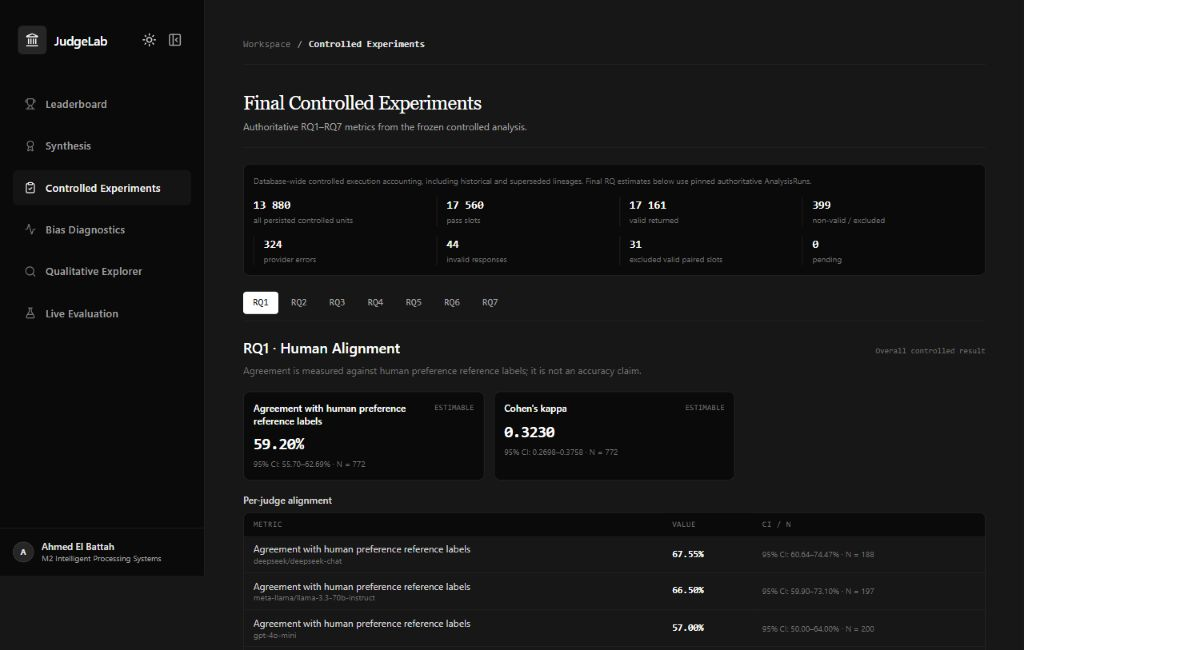
\includegraphics[width=0.94\textwidth]{figures/controlled-results-ui.png}
\caption{Local Controlled Experiments interface captured without any provider request. It displays analysis-run-pinned final evidence and distinguishes coverage from excluded slots.}
\label{fig:controlled-results-ui}
\end{figure}

\section{API safety and analysis-run selection}

The controlled-results API is deliberately DB-authoritative. It selects a uniquely matching analysis run by expected identity and required provenance, validates required metrics and confidence intervals, and fails closed if the selection is missing, duplicate, wrong-role, or malformed. RQ7 exposes DUAL\_SWAP as PRIMARY and Multi-Judge Consensus as SECONDARY. It does not emit a synthetic direct DUAL\_SWAP-versus-Multi-Judge delta. Focused tests cover missing run, duplicate run, wrong RQ, wrong role, missing metrics, missing confidence intervals, and missing provenance cases.

This design is a reproducibility feature as much as a software-engineering feature. A hard-coded front-end number would be easy to display but hard to audit. A fail-closed response makes an evidence break visible. The frontend uses API-derived values and presents the two mitigation families as complementary, each with its own comparator boundary.

\section{Live Evaluation isolation}

Live Evaluation is a local manual sandbox. Its provider execution gate is server-side and controlled through \texttt{ENABLE\_LIVE\_SANDBOX\_PROVIDER\_CALLS}; the safe example configuration defaults to false. When disabled, execution is rejected before any provider transport. When enabled in a local environment with credentials present, standard, calibrated, and ensemble modes can be used for an ad-hoc manual trial. The UI avoids population-level claims: it reports the current trial, a dual-pass result, or an order-sensitive change observed in this trial. It does not call a single trial a model-level bias finding or empirical debiasing result.

Most importantly, live results are classified separately from historical exploratory telemetry and frozen controlled evidence. They cannot modify final analysis runs or feed the final API. This is tested as a telemetry-isolation invariant.

\section{Reproducibility packages}

The repository preserves a historical Phase 11 evidence package and newer source-corrected and release-v4 packages. Historical artifacts are not deleted or silently reinterpreted; the report states which final source-corrected artifact is authoritative. Frozen verifier scripts check checksums, inventory, provenance, and result consistency. Release snapshots provide database restoration and API reconciliation checks. These procedures can be run provider-free because they validate persisted evidence rather than generating new judge outcomes.

\begin{table}[H]
\centering
\caption{Reproducibility layers and their roles.}
\label{tab:repro-layers}
\begin{tabularx}{\textwidth}{@{}p{0.26\textwidth}X@{}}
\toprule
Layer & Role \\
\midrule
Canonical data & Exact source text, question identity, answer identity, and source hashes.\\
Controlled database & Units, passes, attempts, terminal states, and analysis-run records.\\
Analysis artifact & Frozen estimator output, seeds, bootstrap policy, lineages, and numerical results.\\
Evidence packages & Checksums, inventories, and immutable copies for audit/reconstruction.\\
Release snapshots & Fresh database restore and API reconciliation without provider calls.\\
Automated tests & Route fail-closed behaviour, provenance, controlled metrics, and telemetry isolation.\\
\bottomrule
\end{tabularx}
\end{table}

\section{Provider-free verification workflow}

A fresh verification workflow begins by checking the canonical data hash and the source-corrected artifact identity. It then verifies the release package, restores the disposable release database, starts the backend against that restored database, and calls the controlled-results endpoint. The returned RQ1--RQ6 values and the two RQ7 components are reconciled with their authoritative analysis runs. Finally, the frontend tests, linting, type checks, and production build ensure the interface remains an accurate consumer of the API.

This workflow is intentionally capable of running without provider credit. It verifies the scientific evidence already collected, not the availability or present-day behavior of a provider. A later researcher can therefore distinguish a reproducibility failure from an execution-cost constraint.

\section{Repository organization}

The final repository keeps top-level backend essentials and semantic packages for API, core, data, evaluation, analysis, experiments, multi-judge work, release tooling, and historical lineage. A small set of compatibility shims is retained only where immutable frozen verification paths demonstrably require a legacy import path. Standalone historical tools live outside active runtime areas. This organization makes the public workflow easier to identify while preserving the scripts needed to explain or validate historical and corrected releases.

\section{Ethical and operational considerations}

Automated judging affects which systems are selected, tuned, or trusted. Overstating an evaluator's reliability can therefore propagate unfair or low-quality choices. The practical safeguards in this project are provenance, fail-closed API selection, visible coverage, no implicit imputation, and separation of exploratory/manual interaction from final evidence. These safeguards do not make an evaluator neutral or universally reliable. They make the limits of the reported result inspectable.
